In order to evaluate and validate the approach proposed in this paper, we have
conducted experiments on simulated and real-world data. Simulated data have been
generated from greyscale images, where each pixel corresponds to a measurement.
Data are contaminated with Gaussian noise in all directions. Real-world data
have been acquired with a nodding laser range-finder setup. Two different lasers
have been mounted, namely a SICK LMS-200 and an Hockuyo UTM-30LX.

%Before we proceed with the actual results, we clarify the detection of curb
%points and the creation of a traversability map. In order to extract the curb
%points from the DEM, we use the MAP solution to the labeling proposed by the
%CRF. An edge between two neighboring cells is considered as a curb whenever they
%are labeled differently. For the traversability map, we assign a cost to each
%curb point, which represents the cost of traversing this edge. We compute the
%maximal gradient of the 8-neighborhood $N_8$ as

%\begin{equation}
%\label{8-neighborhood}
%g_{max}=\max_{(i,j)\in N_8}|h_i-h_j|.
%\end{equation}

%The traversability cost $t_{ij}$ for the edge connecting cell $i$ with cell $j$
%is then calculated as

%\begin{eqnarray}
%\label{eqn:traversability}
%t_{ij}(g_{max})=
%\left\{
%\begin{array}{l l}
%0 & \quad \text{if $g_{max}\le c_0$}\\
%g_{max}/c_{max} & \quad \text{if $c_0\le g_{max}\le c_{max}$}\\
%1 & \quad \text{if $c_{max}\le g_{max}$},
%\end{array} \right.
%\end{eqnarray}

%where $c_0$ is the lower boundary and $c_{max}$ the maximal step height the
%system can traverse.

The simulated data allow us to show the pertinence of our algorithm in
particular settings such as a T-junction, where other approaches fail.
Fig.~\ref{fig:t-junction} illustrates such a situation.

\begin{figure}[t]
\centering
\includegraphics[width=\columnwidth]{fig/t-junction.eps}
\caption{Simulated data of a T-junction. Our algorithm is able to recover the
correct curb points and output an adequate traversability map.}
\label{fig:t-junction}
\end{figure}

Experiments on real-world data are reported in Fig.\ref{fig:exp1}-\ref{fig:exp2}
-\ref{fig:exp3}. These demonstrate the validity of our approach.

\begin{figure}[t]
\centering
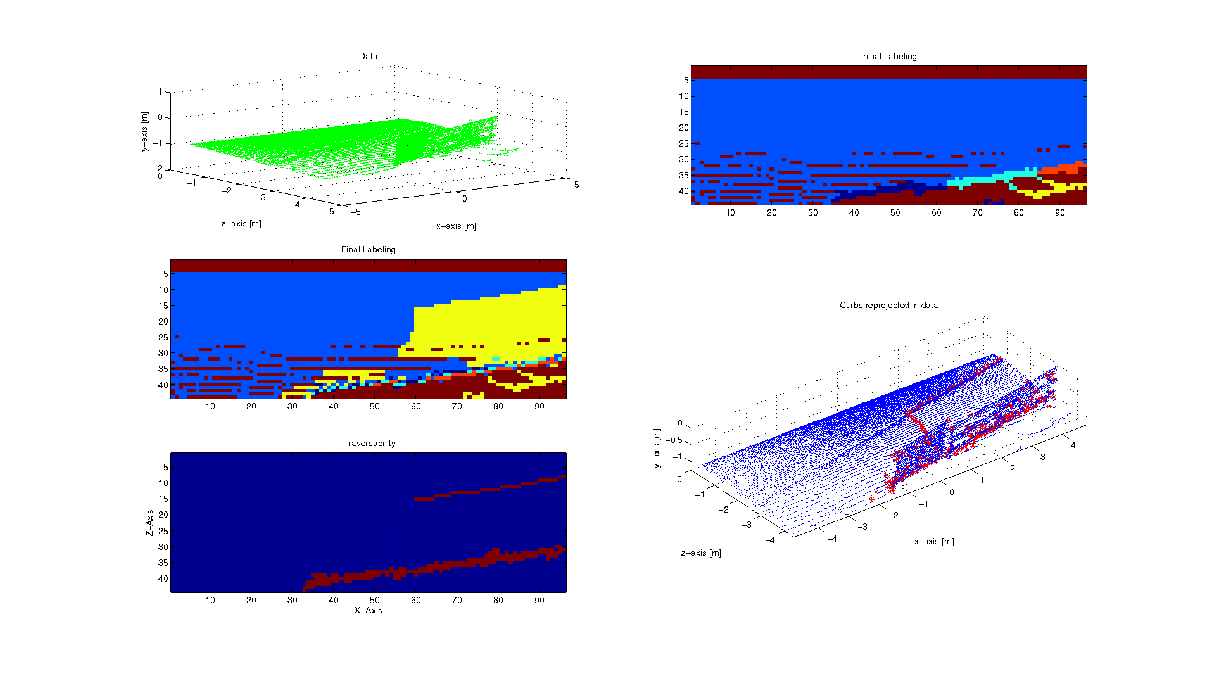
\includegraphics[width=\columnwidth]{fig/exp1.eps}
\caption{Curb detection on real-world data.}
\label{fig:exp1}
\end{figure}

\begin{figure}[t]
\centering
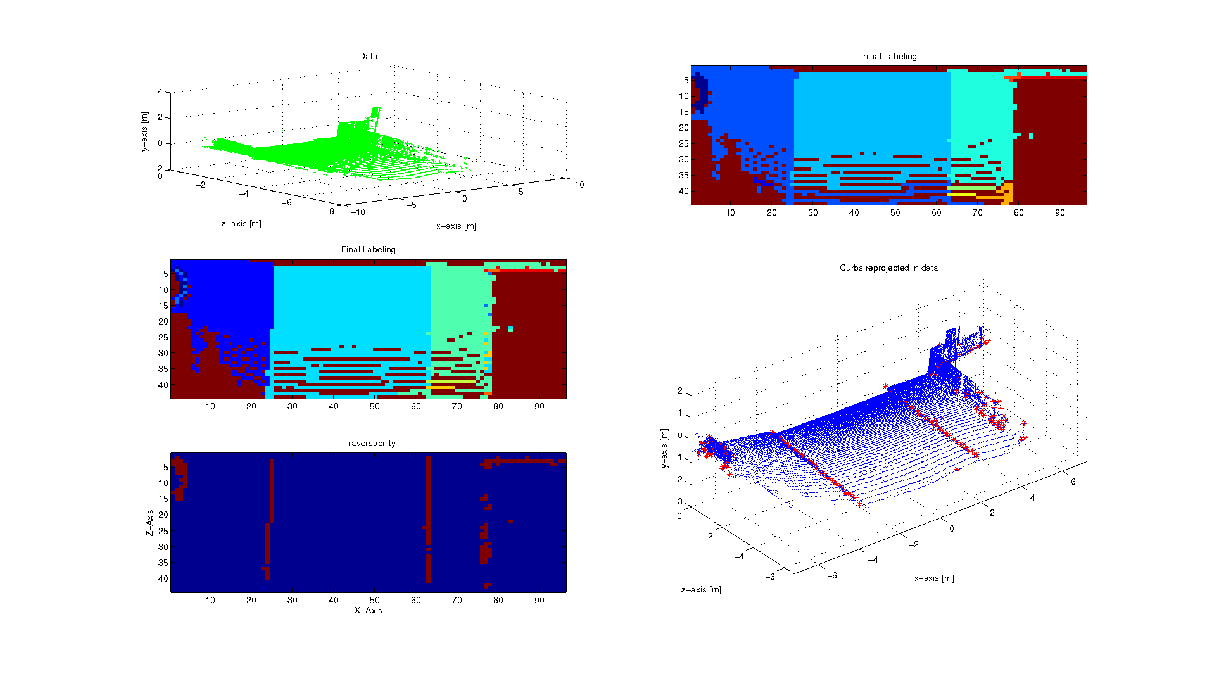
\includegraphics[width=\columnwidth]{fig/exp2.eps}
\caption{Curb detection on real-world data.}
\label{fig:exp2}
\end{figure}

\begin{figure}[t]
\centering
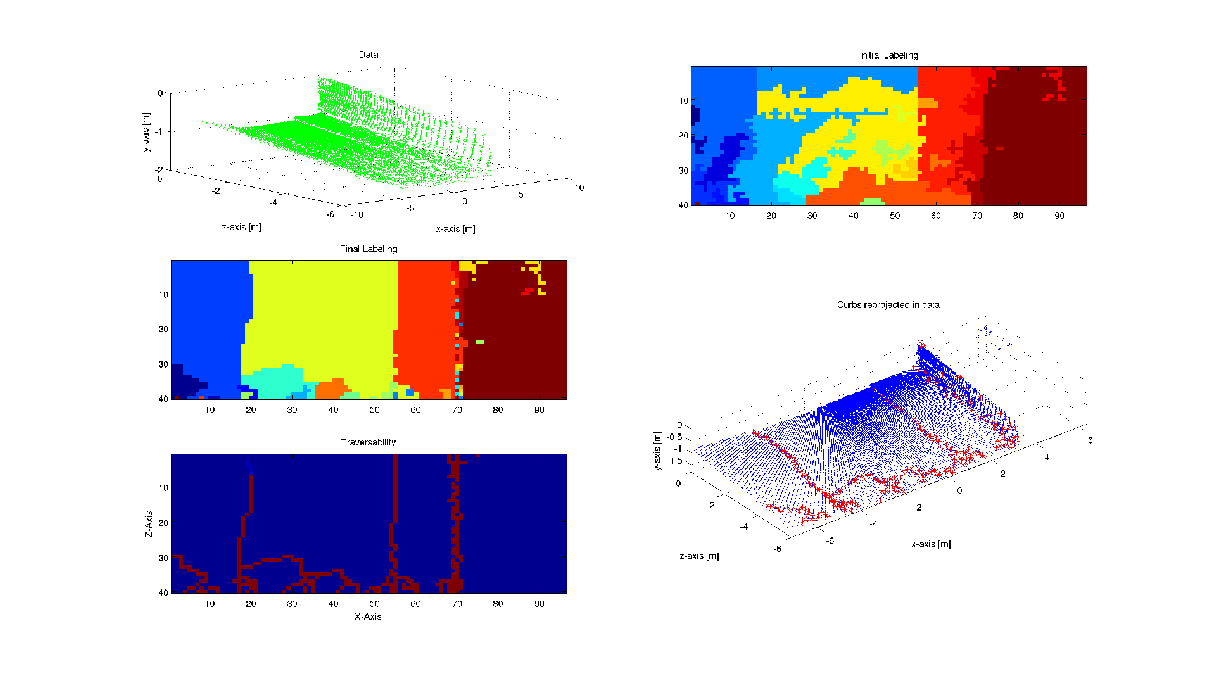
\includegraphics[width=\columnwidth]{fig/exp3.eps}
\caption{Curb detection on real-world data.}
\label{fig:exp3}
\end{figure}
